\documentclass{article}
\usepackage{amsmath}
\usepackage{amssymb}
\usepackage{braket}
\usepackage{changepage}
\usepackage[normalem]{ulem} % for strikeout line
\usepackage{graphicx}
\usepackage{epstopdf}

%-------------------------------------------------------%
\newcounter{pcounter}                                   %
\newenvironment{problem}                                %
{                                                       %
    \stepcounter{pcounter}                              %
    (\arabic{pcounter})                                 %
}{}                                                     %
\newenvironment{solution}                               %
{\textbf{Solution:} \\}{$\blacksquare$\newline}         %
%-------------------------------------------------------%
\newcommand{\leadto}{\Rightarrow}                       %
\newcommand{\domR}{\mathbb{R}}                          %
\newcommand{\domS}{\mathbb{S}}                          %
\newcommand{\abss}[1]{\| #1 \|}                         %
\newcommand{\tr}[1]{\textbf{tr}(#1)}                    %
\newcommand{\vecOne}{\textbf{1}}                        %
%-------------------------------------------------------%

\begin{document}

%------------------- The Title -------------------%
\parindent 0in
\parskip 1em
\title{COMP9602 Assignment 3 Solution Sheet}
\author{3030058647, HONG Yuncong}
\maketitle

%=============== Problem Description =============%
You are given the following convex optimization problem:
\begin{align*}
    minimize\ &f(x) = \sum_{i=1}^n (1+x_i)^a log(1+x_i) \\
    subject\ to \ 
        &b^T x \leq c \\
        &\vecOne^T x \geq d \\
        &x \succeq 0
\end{align*}
where the variable is $x \in \domR^n$, and we have $a \geq 2$, $b \in \domR_+^n$, $c \in \domR$, $d \in \domR$.

%=================== Problem 1 ===================%
\begin{problem}
    Derive a \textbf{partial Lagrange dual} of the above problem, with partial Lagrangian relaxation that \textbf{only relaxes constraint $b^T x \leq c$} when computing the Lagrangian. Note that you do not need to derive the explicit form of the partial lagrange dual function $\tilde{g}(\lambda)$, but just need to give all the steps to derive that partial Lagrange dual, and give the dual problem using $\tilde{g}(\lambda)$ as the objective function. This part (1) is to facilitate your design of the \textbf{projected subgradient algorithm} for dual problem in part (2).
\end{problem}

\begin{solution}
    Firstly, we write up the partial Lagrange formula as:
    \begin{align*}
        &L(x, \lambda) = f(x) + \lambda (b^T x - c) \\
        s.t.\ 
            &\vecOne^T x \geq d \\
            &x \succeq 0
    \end{align*}
    $\tilde{g}(\lambda) = \inf\limits_{x \in C} L(x, \lambda)$, where $C = \{x \in \domR^n | \vecOne^T x \geq d, x \succeq 0\}$
    
    And then we could reformulate the primal problem into a partial Lagrange dual problem:
    \begin{align*}
        &\max\limits_{\lambda \in \domR_+} \tilde{g}(\lambda) \\
        s.t.\ 
        &\vecOne^T x \geq d \\
        &x \succeq 0
    \end{align*}
\end{solution}

%=================== Problem 2 ===================%
\begin{problem}
    Suppose strong duality holds for this convex problem. Design a \textbf{projected subgradient algorithm} for dual problem to solve this optimization problem (i.e., derive $x^*$), based on the partial Lagrange dual problem you have obtained in part (1). You should clearly describe \textbf{how you derive or update the primal and dual variable values} in each iteration of the algorithm.
\end{problem}

\begin{solution}
    The subgradient descent method for a dual problem si always feasible, for $g(\lambda)$ is always concave over $\lambda \in \domR_+$;\\
    But for the partial Lagrangian equation, when we find the subgradient at certain $\lambda$, we need to solve the optimization problem: $\inf\limits_{x \in C} \tilde{g(\lambda)}$, with constraint area.

    Here we take it as a a sub-problem; and as it's one differentialble function, we try to solve this subproblem using simple gradient descent method with projection.

    The whole algorithm designed follow:

    \textbf{Repeat}
    \begin{adjustwidth}{0.5cm}{}
        1. Choose $\lambda^{(1)}$ initially, with $k=1$ \\
        2. $x^{(k)} = arg\min\limits_z\ (f(z) + \lambda^{(k)} (b^Tz-c))$, where $C = \{x \in \domR^n | \vecOne^T x \geq d, x \succeq 0\}$; solved as a subproblem by \textbf{projected gradient descent method}:
        \begin{adjustwidth}{0.5cm}{}
            \textbf{Repeat}\\
            a) Choose $x^{(k_i)}$ initially, with $i:=1$ \\
            b) Find gradient $\Delta{x} := \nabla_x g(x^{(k_i)}, \lambda)$ \\
            c) Choose step size $t^{(k_i)}$\\
            d) Update $x^{(k_i+1)} := P_C [x^{(k_i)} + t^{(k_i)} * \Delta{x}]$, where $C = \{x \in \domR^n | \vecOne^T x \geq d, x \succeq 0\} \Rightarrow \{x \in \domR^n | \sum{|x_i|} \geq d\}$; P is Euclidean projected function (Since the constrained space C is outside one simplex, the projection should be on the nearest plane of n planes) \\
            \textbf{Until} stopping criteria $\epsilon_2$ is satisfied.
        \end{adjustwidth}
        3. choose subgradient with $h^{(k)} = b^T x^{(k)} - c$ \\
        4. choose step size $\alpha^{(k)}$; \\
        5. $\lambda_{i}^{(k+1)} = [\lambda_{i}^{(k)} + \alpha_k (b^T x^{(k)} - c)]_+ $
    \end{adjustwidth}
    \textbf{Until} stopping criteria $\epsilon_1$ is satisfied.

\end{solution}

%=================== Problem 3 ===================%
\begin{problem}
    Generate a random instance of the problem with $n = 10$ and $a = 3$. Implement Matlab or python code to solve the problem instance you have created using the algorithm you disigned in (2), with the constant step size rule (you can set the constant). Give the optimal solution of the problem instance that your implementation achieves. \\
    \textit{Hint}: To generate some random problem data, i.e., $b,c,d$, we recommend the following approach. First, generate $b$ randomly. Then generate a random positive vector $x_0$, and find a $c$ and $d$ such that $c > b^T x_0$ and $d < \vecOne^T x_0$. (This ensure that the problem is strictly feasible)
\end{problem}

\begin{solution}
    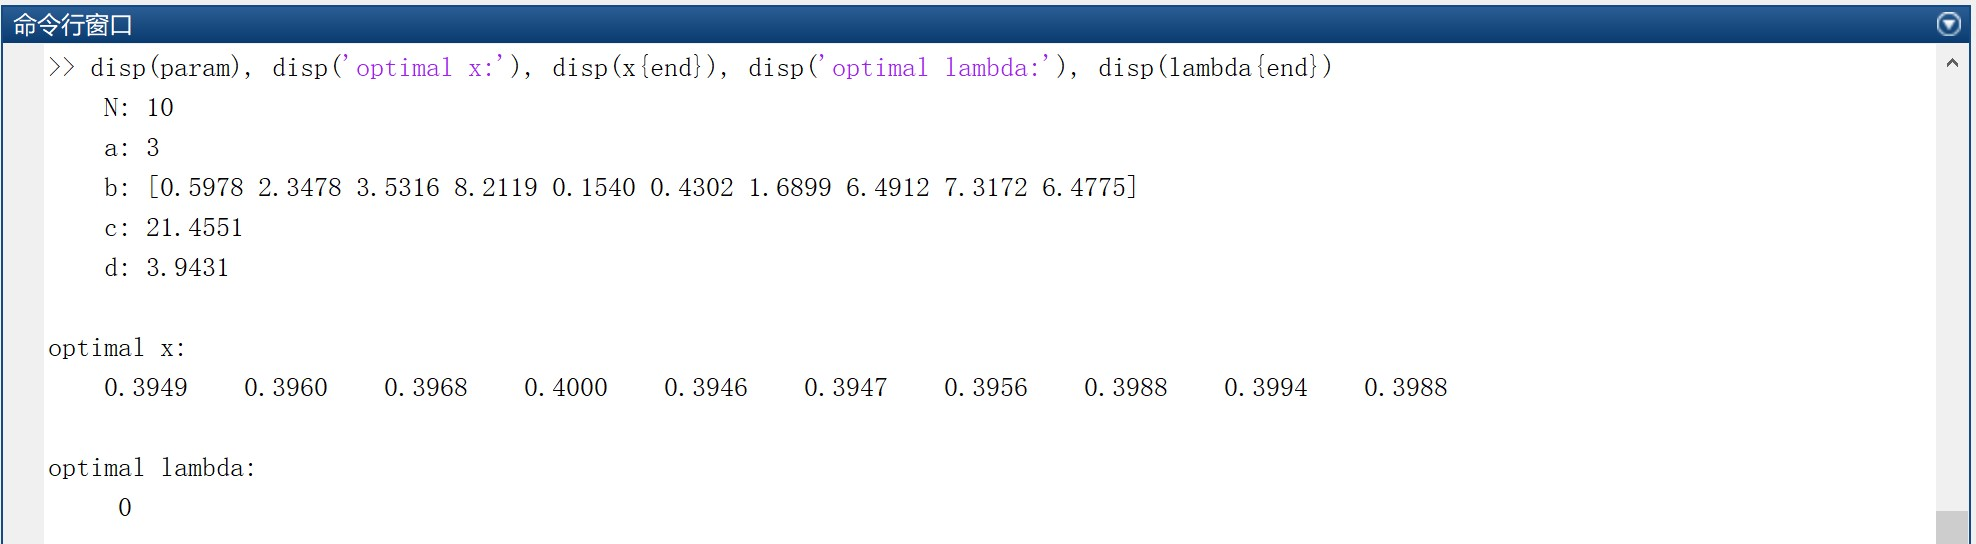
\includegraphics[width=1.0\textwidth]{img/a2+3.jpg}
\end{solution}

%=================== Problem 4 ===================%
\begin{problem}
    For the generated problem instance in (3), use some built-in library or package (e.g., cvx for Matlab, scipy.optimize for Python) to find the optimal value of the problem, $f^*$. Then based on your implementation in (3), plot $f(\tilde{x}^{(k)}) - f^*$ versus iteration number $k$, where $\tilde{x}^{(k)}$ is a nearby feasible point for $x^{(k)}$.
\end{problem}

\begin{solution}
    We could simply solve this problem with built-in library \textit{fmincon}, and have: $x^* = d/n$ for this optimization problem, and the optimization value is $f(x^*)$. (the code is in \textit{script.m}) \\
    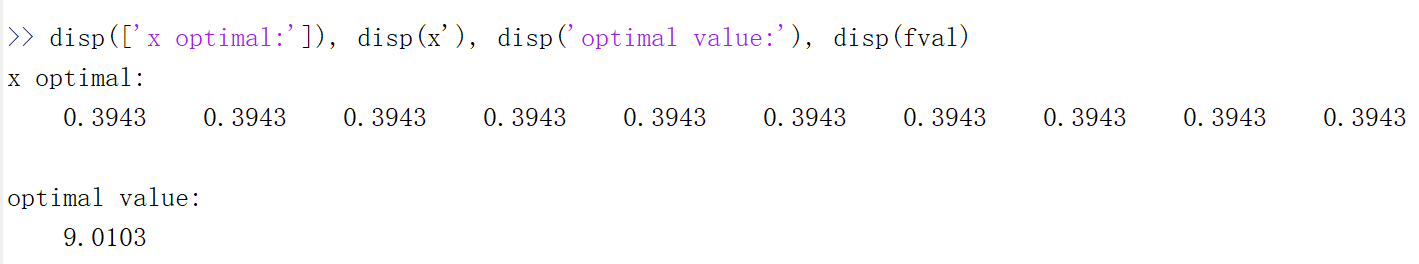
\includegraphics[width=1.0\textwidth]{img/a2+4(1).png}

    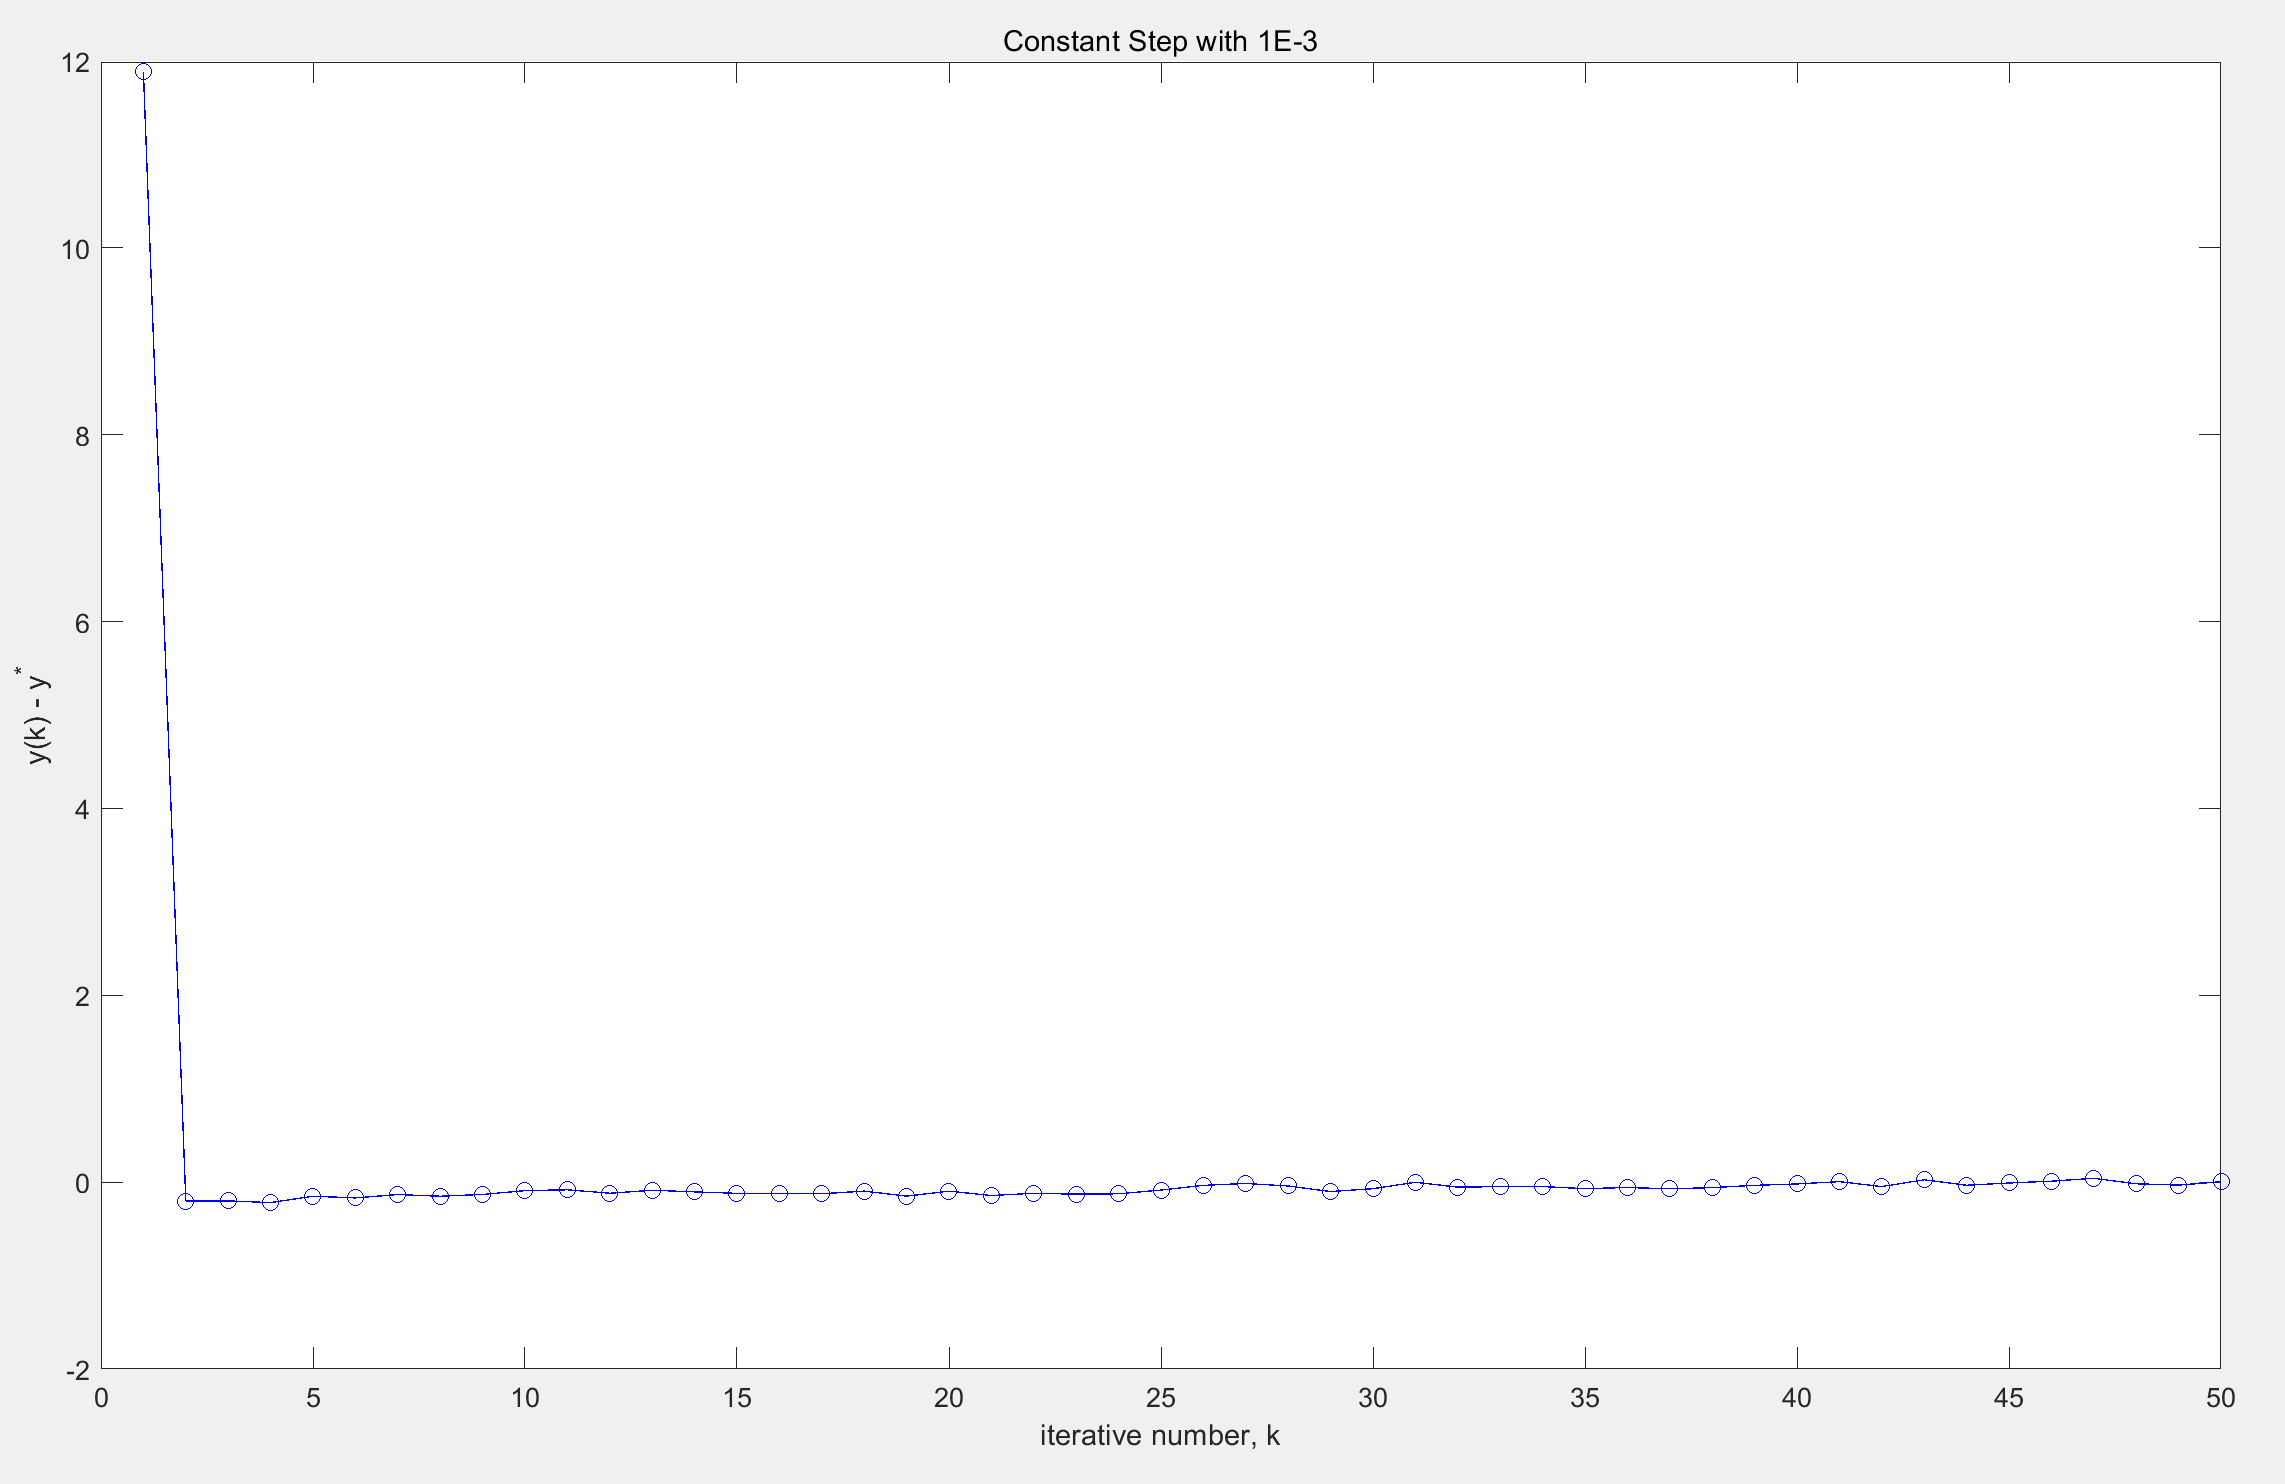
\includegraphics[width=1.0\textwidth]{img/a3+6(1).png}

\end{solution}

%=================== Problem 5 ===================%
\begin{problem}
    For the gerated problem instance in (3), plot a figure to show the upper and lower bounds of the optimal value, i.e., $f(\tilde{x}^{(k)})$ and $\tilde{g}(\lambda^{(k)})$, versus iteration number k.
\end{problem}

\begin{solution}
    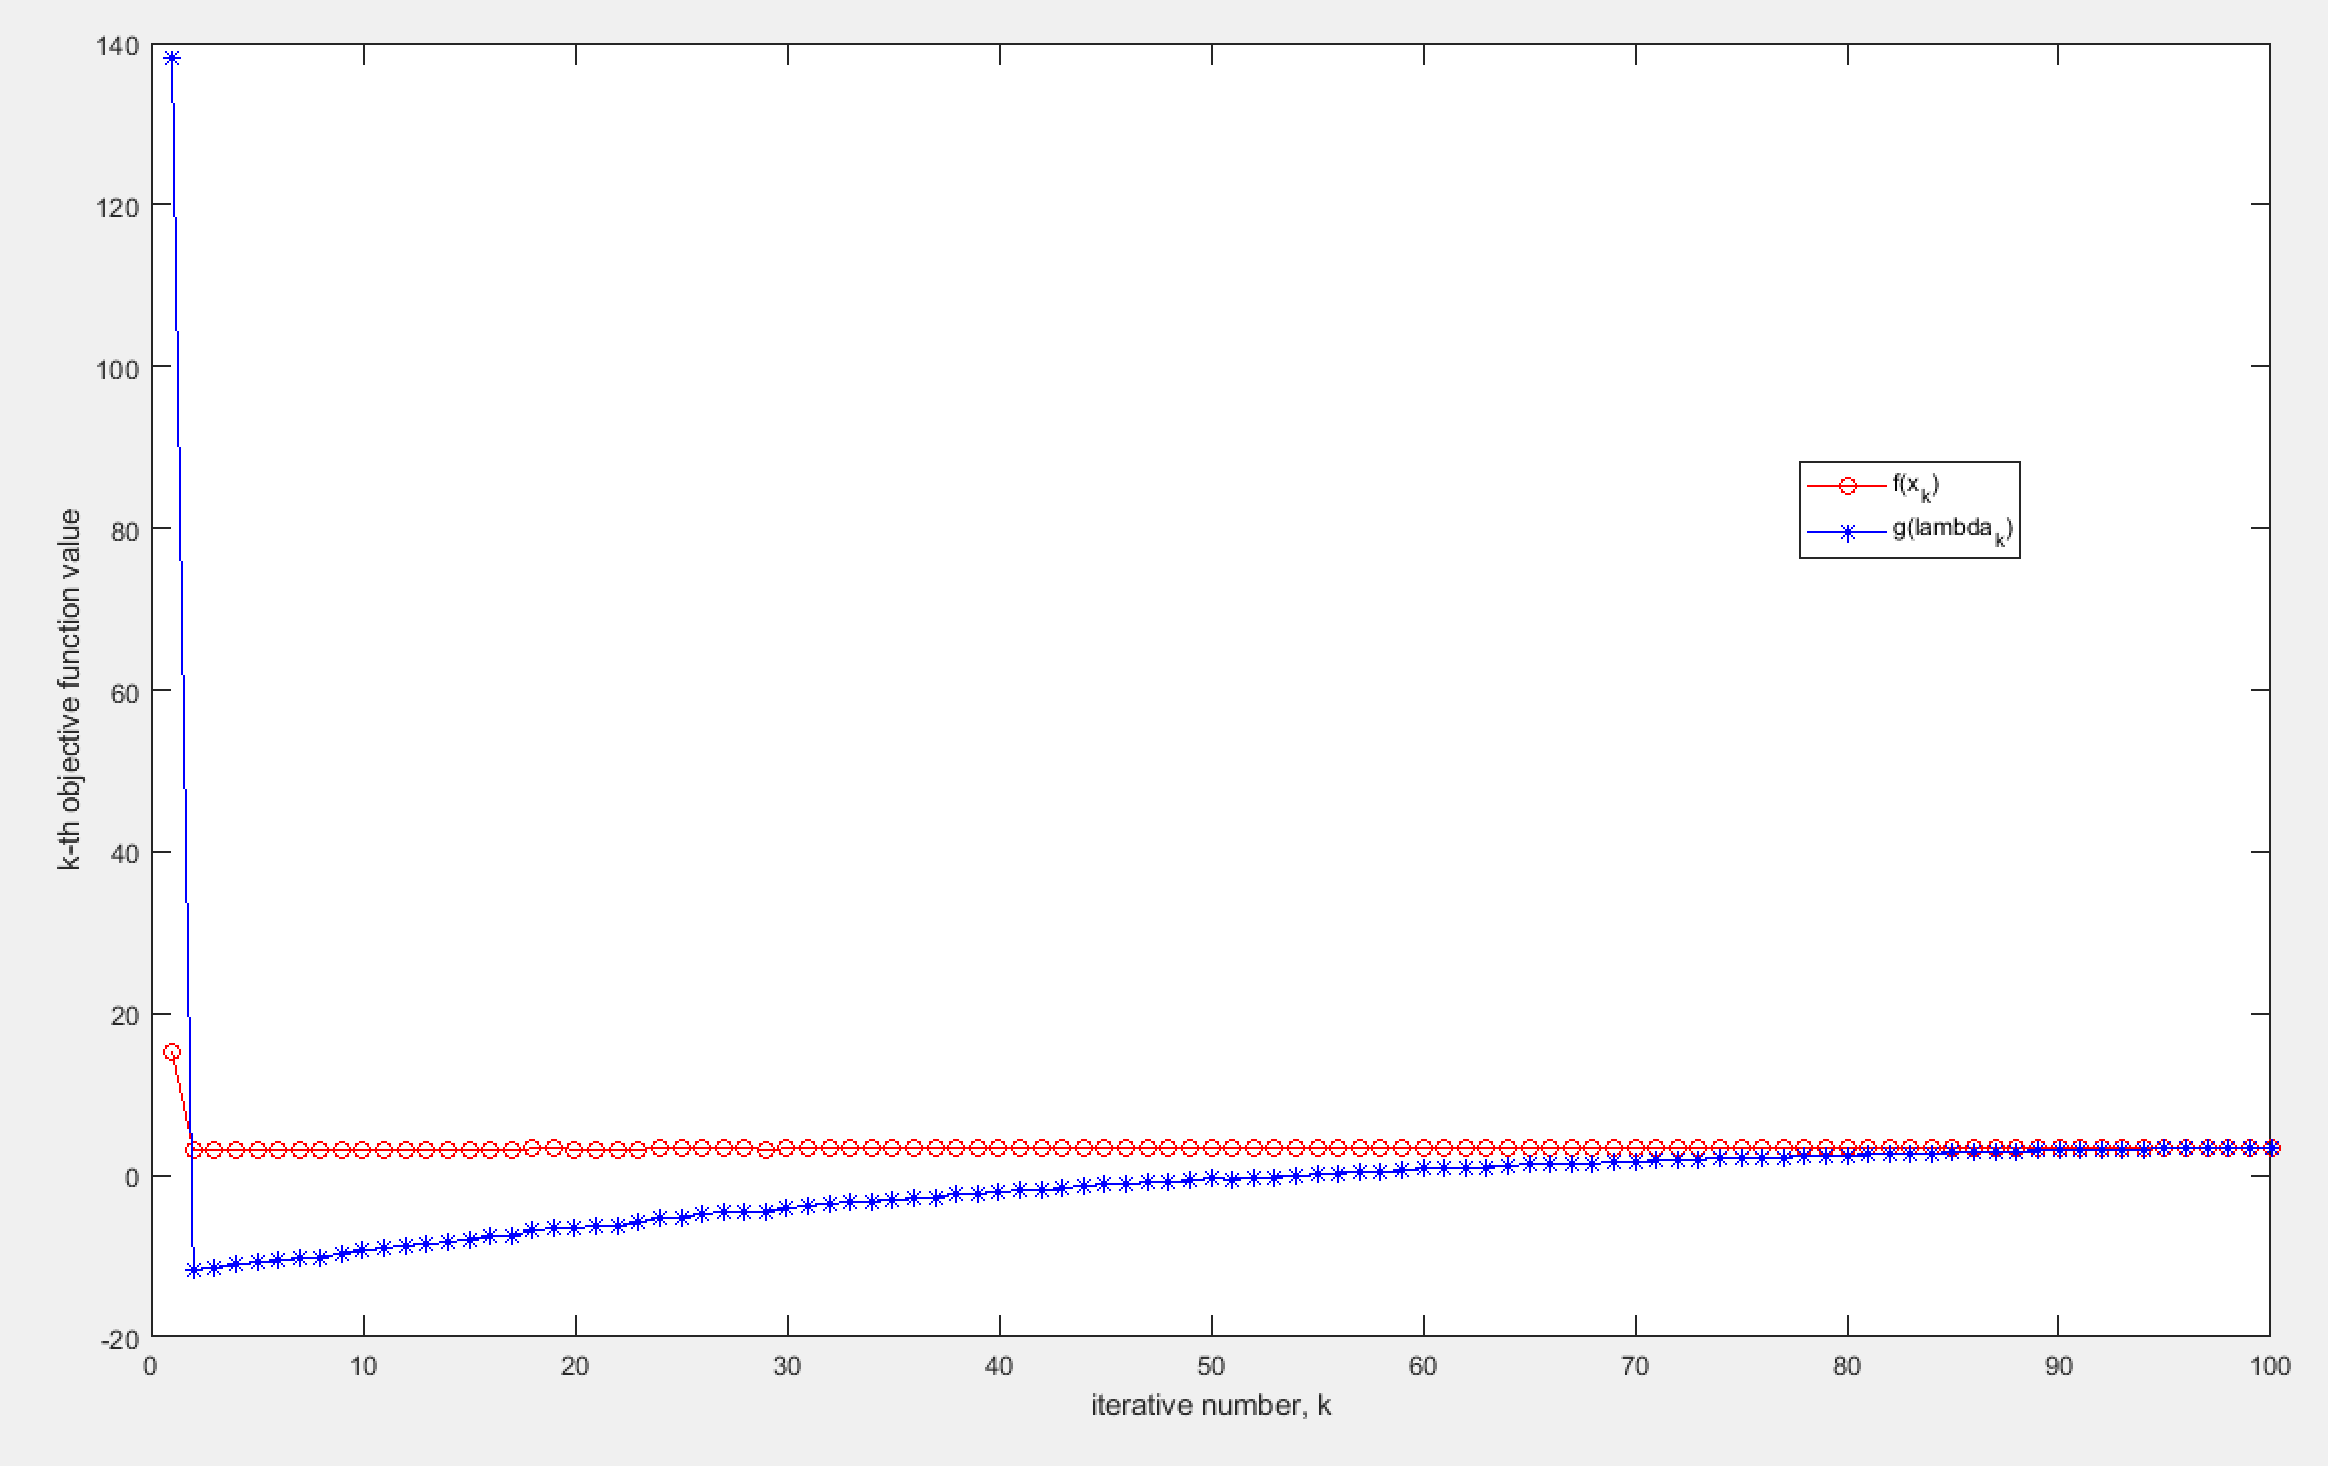
\includegraphics[width=1.0\textwidth]{img/a2+5.png}
\end{solution}

%=================== Problem 6 ===================%
\begin{problem}
    Based on (4), $f(\tilde{x}^{(k)}) - f^*$ versus iteration number $k$, using other step size rules, i.e., constant step length, square summable but nonsummable (use $\alpha_k = \frac{a}{b+k}$), nonsummable diminishing (use $\alpha_k = \frac{1}{\sqrt{k}}$), and the Polyak step size. Draw four curves in the figure correspoding to the four rules; you can set the constants in the step size rules, i.e., $\gamma, a, b$, at your choice.
\end{problem}

\begin{solution}
    Constant step: \\
    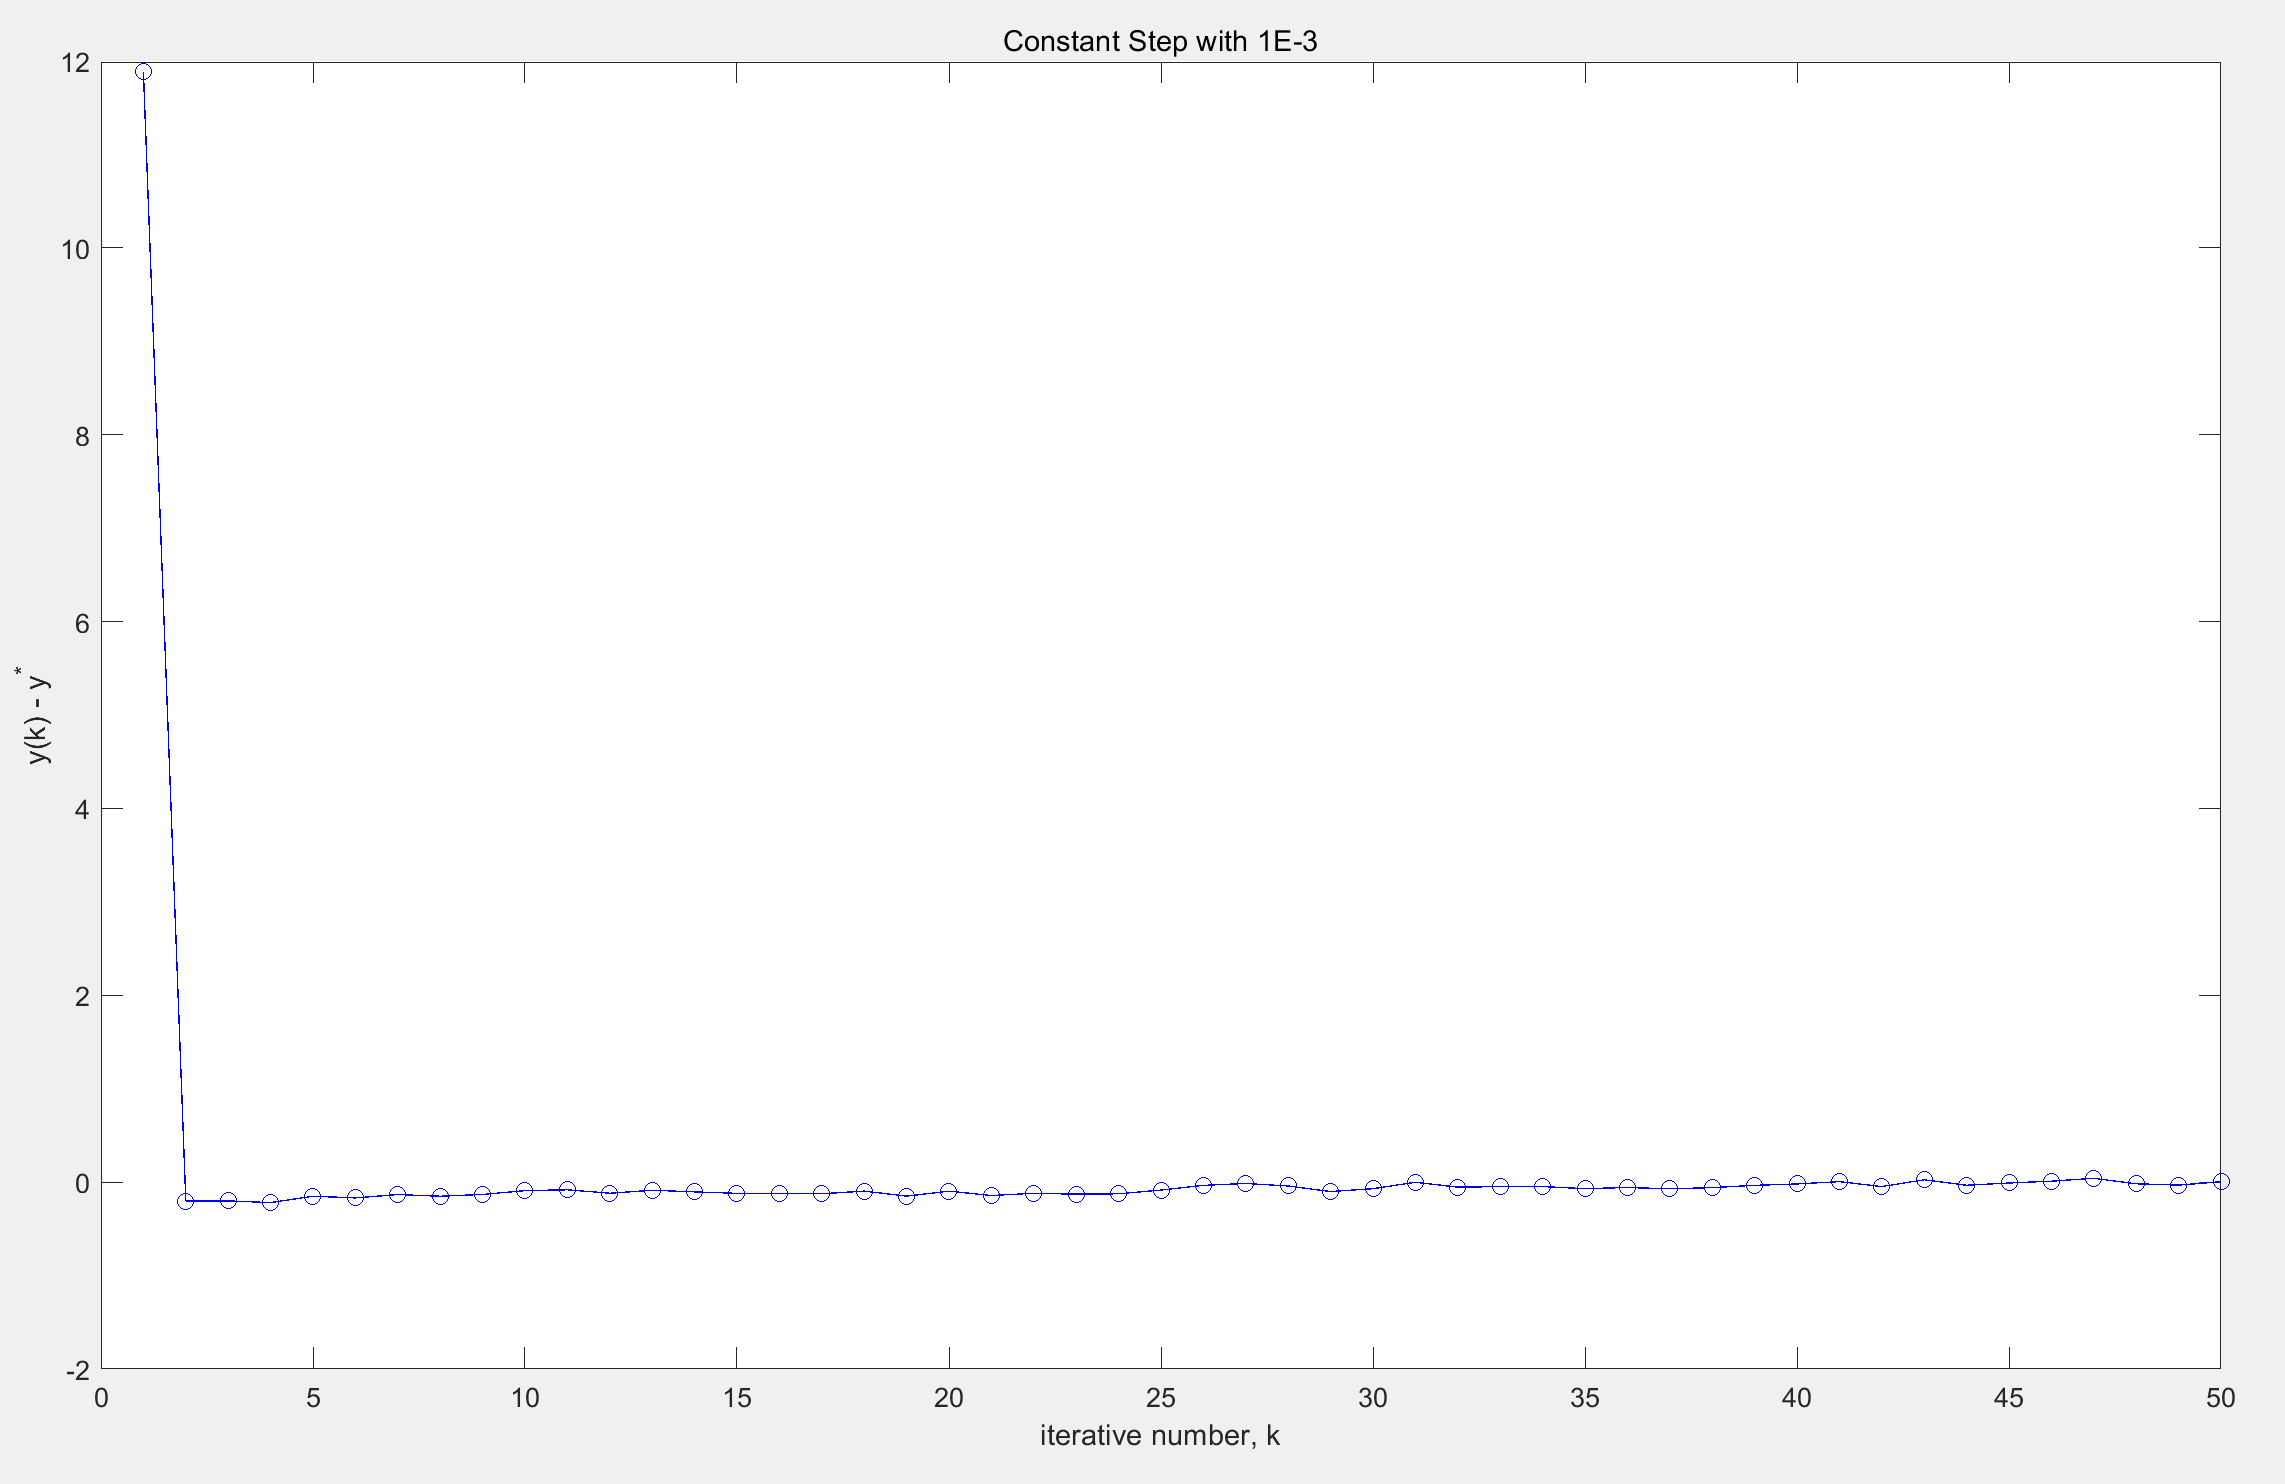
\includegraphics[width=1.0\textwidth]{img/a3+6(1).png}

    Square summable but nonsummable step: \\
    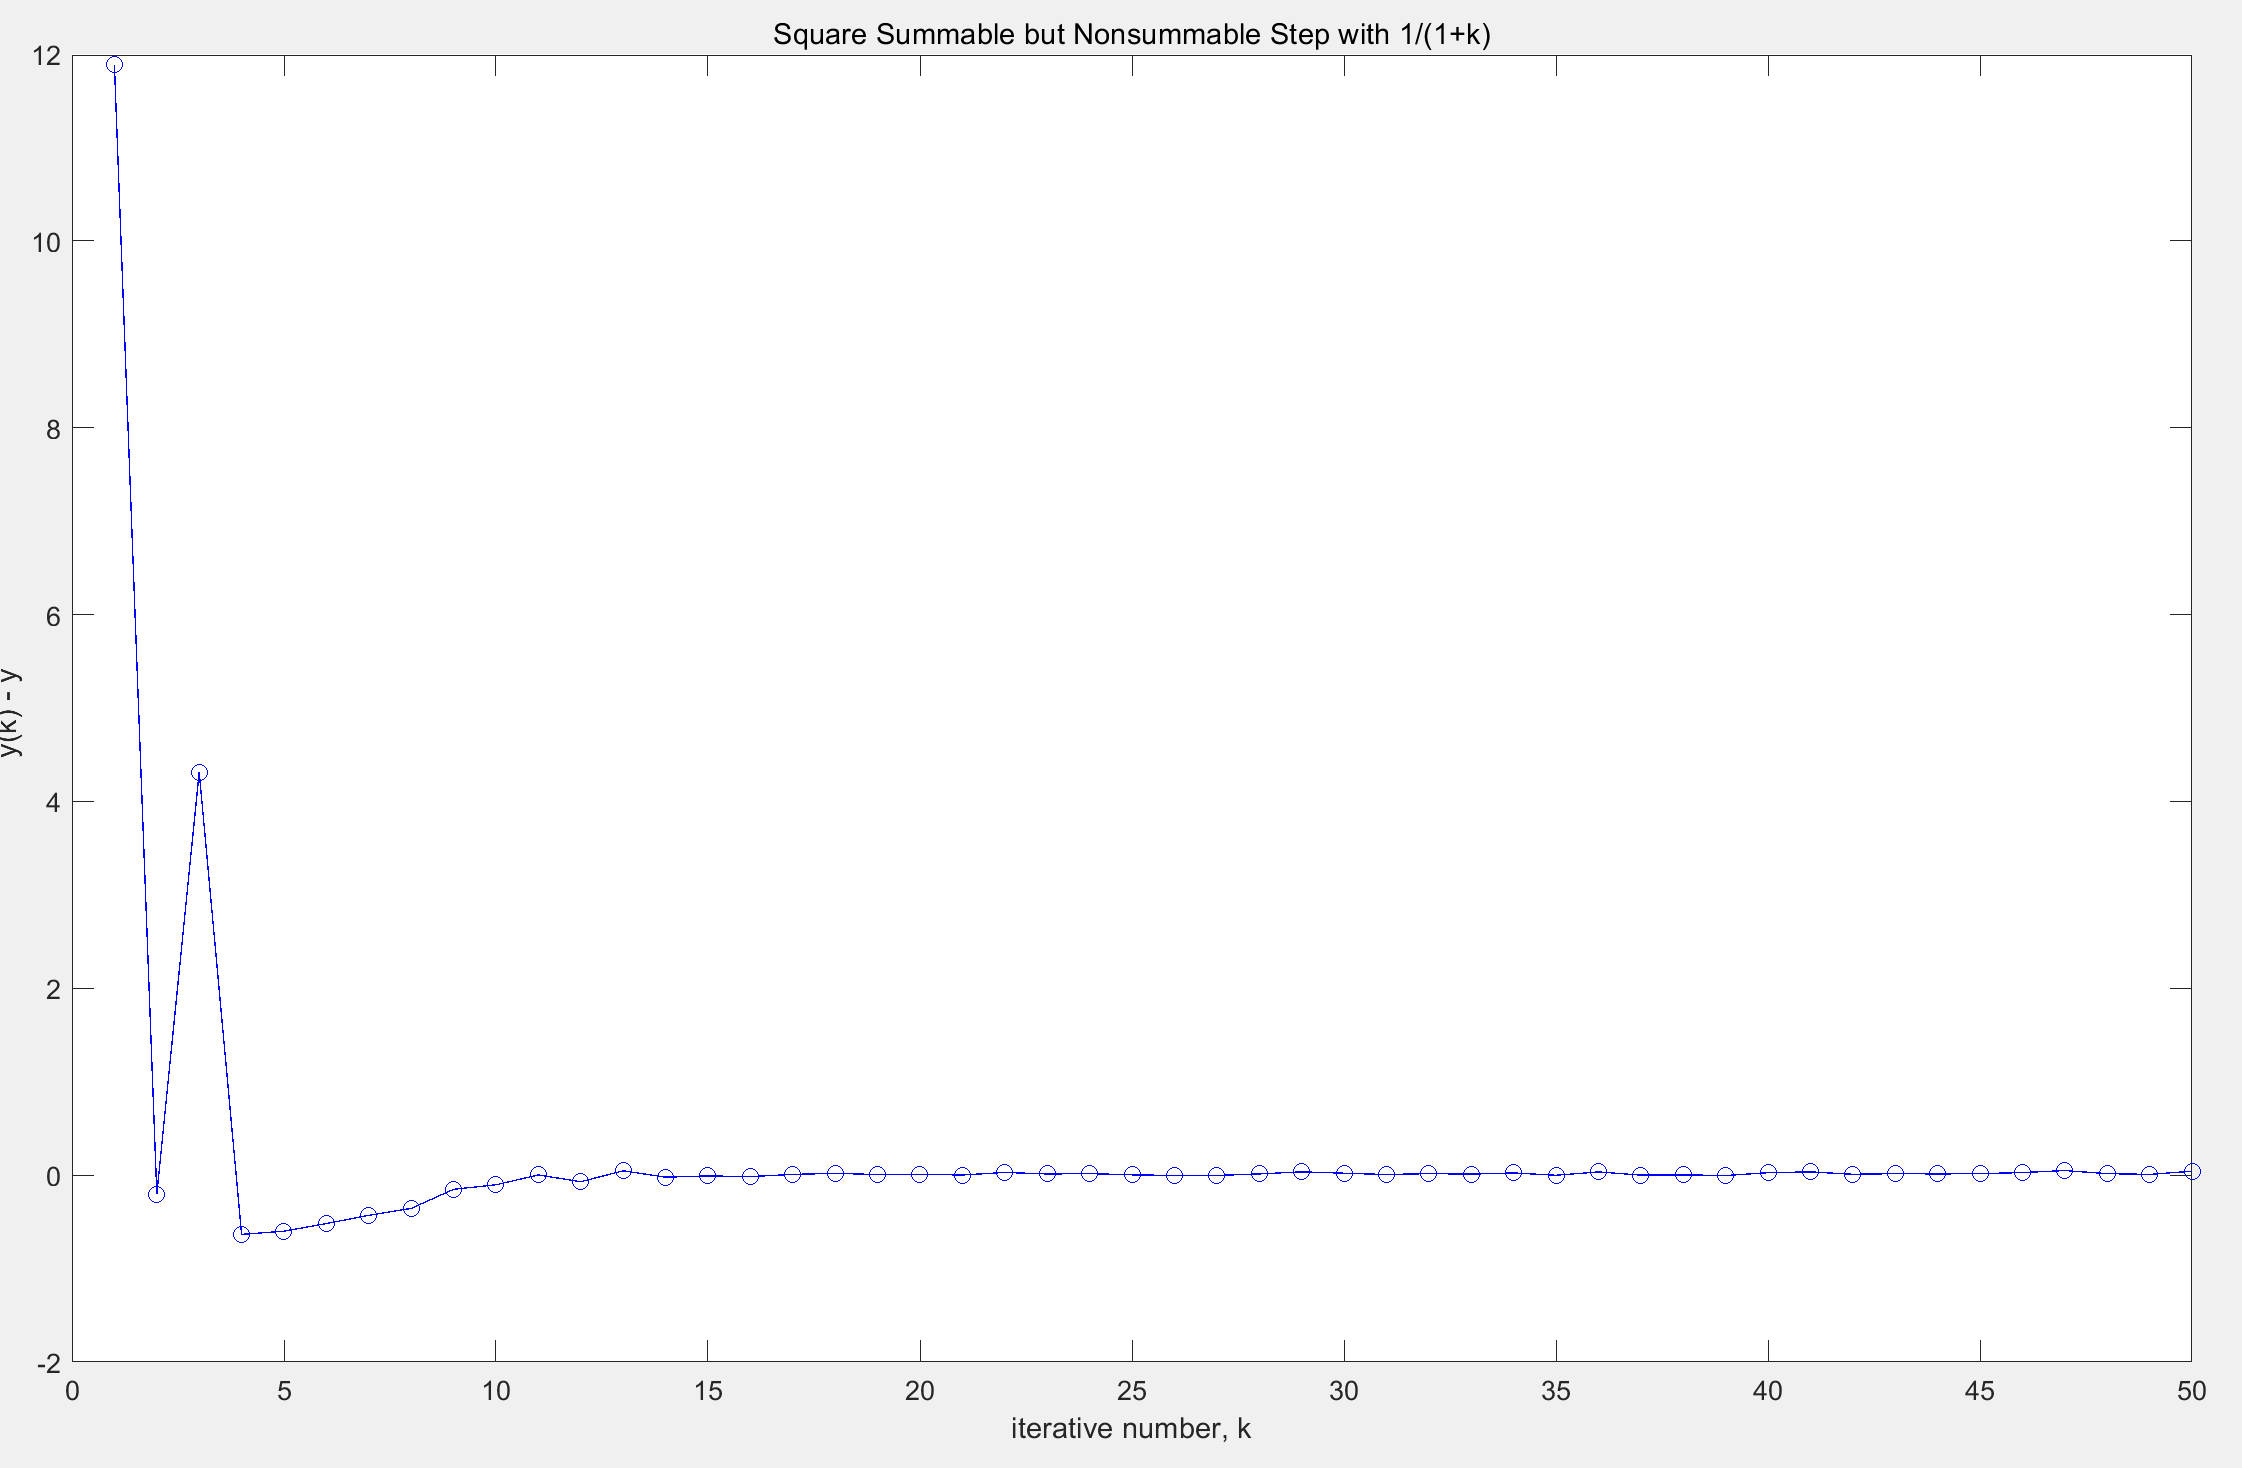
\includegraphics[width=1.0\textwidth]{img/a3+6(2).png}

    Nonsummable diminishing step: \\
    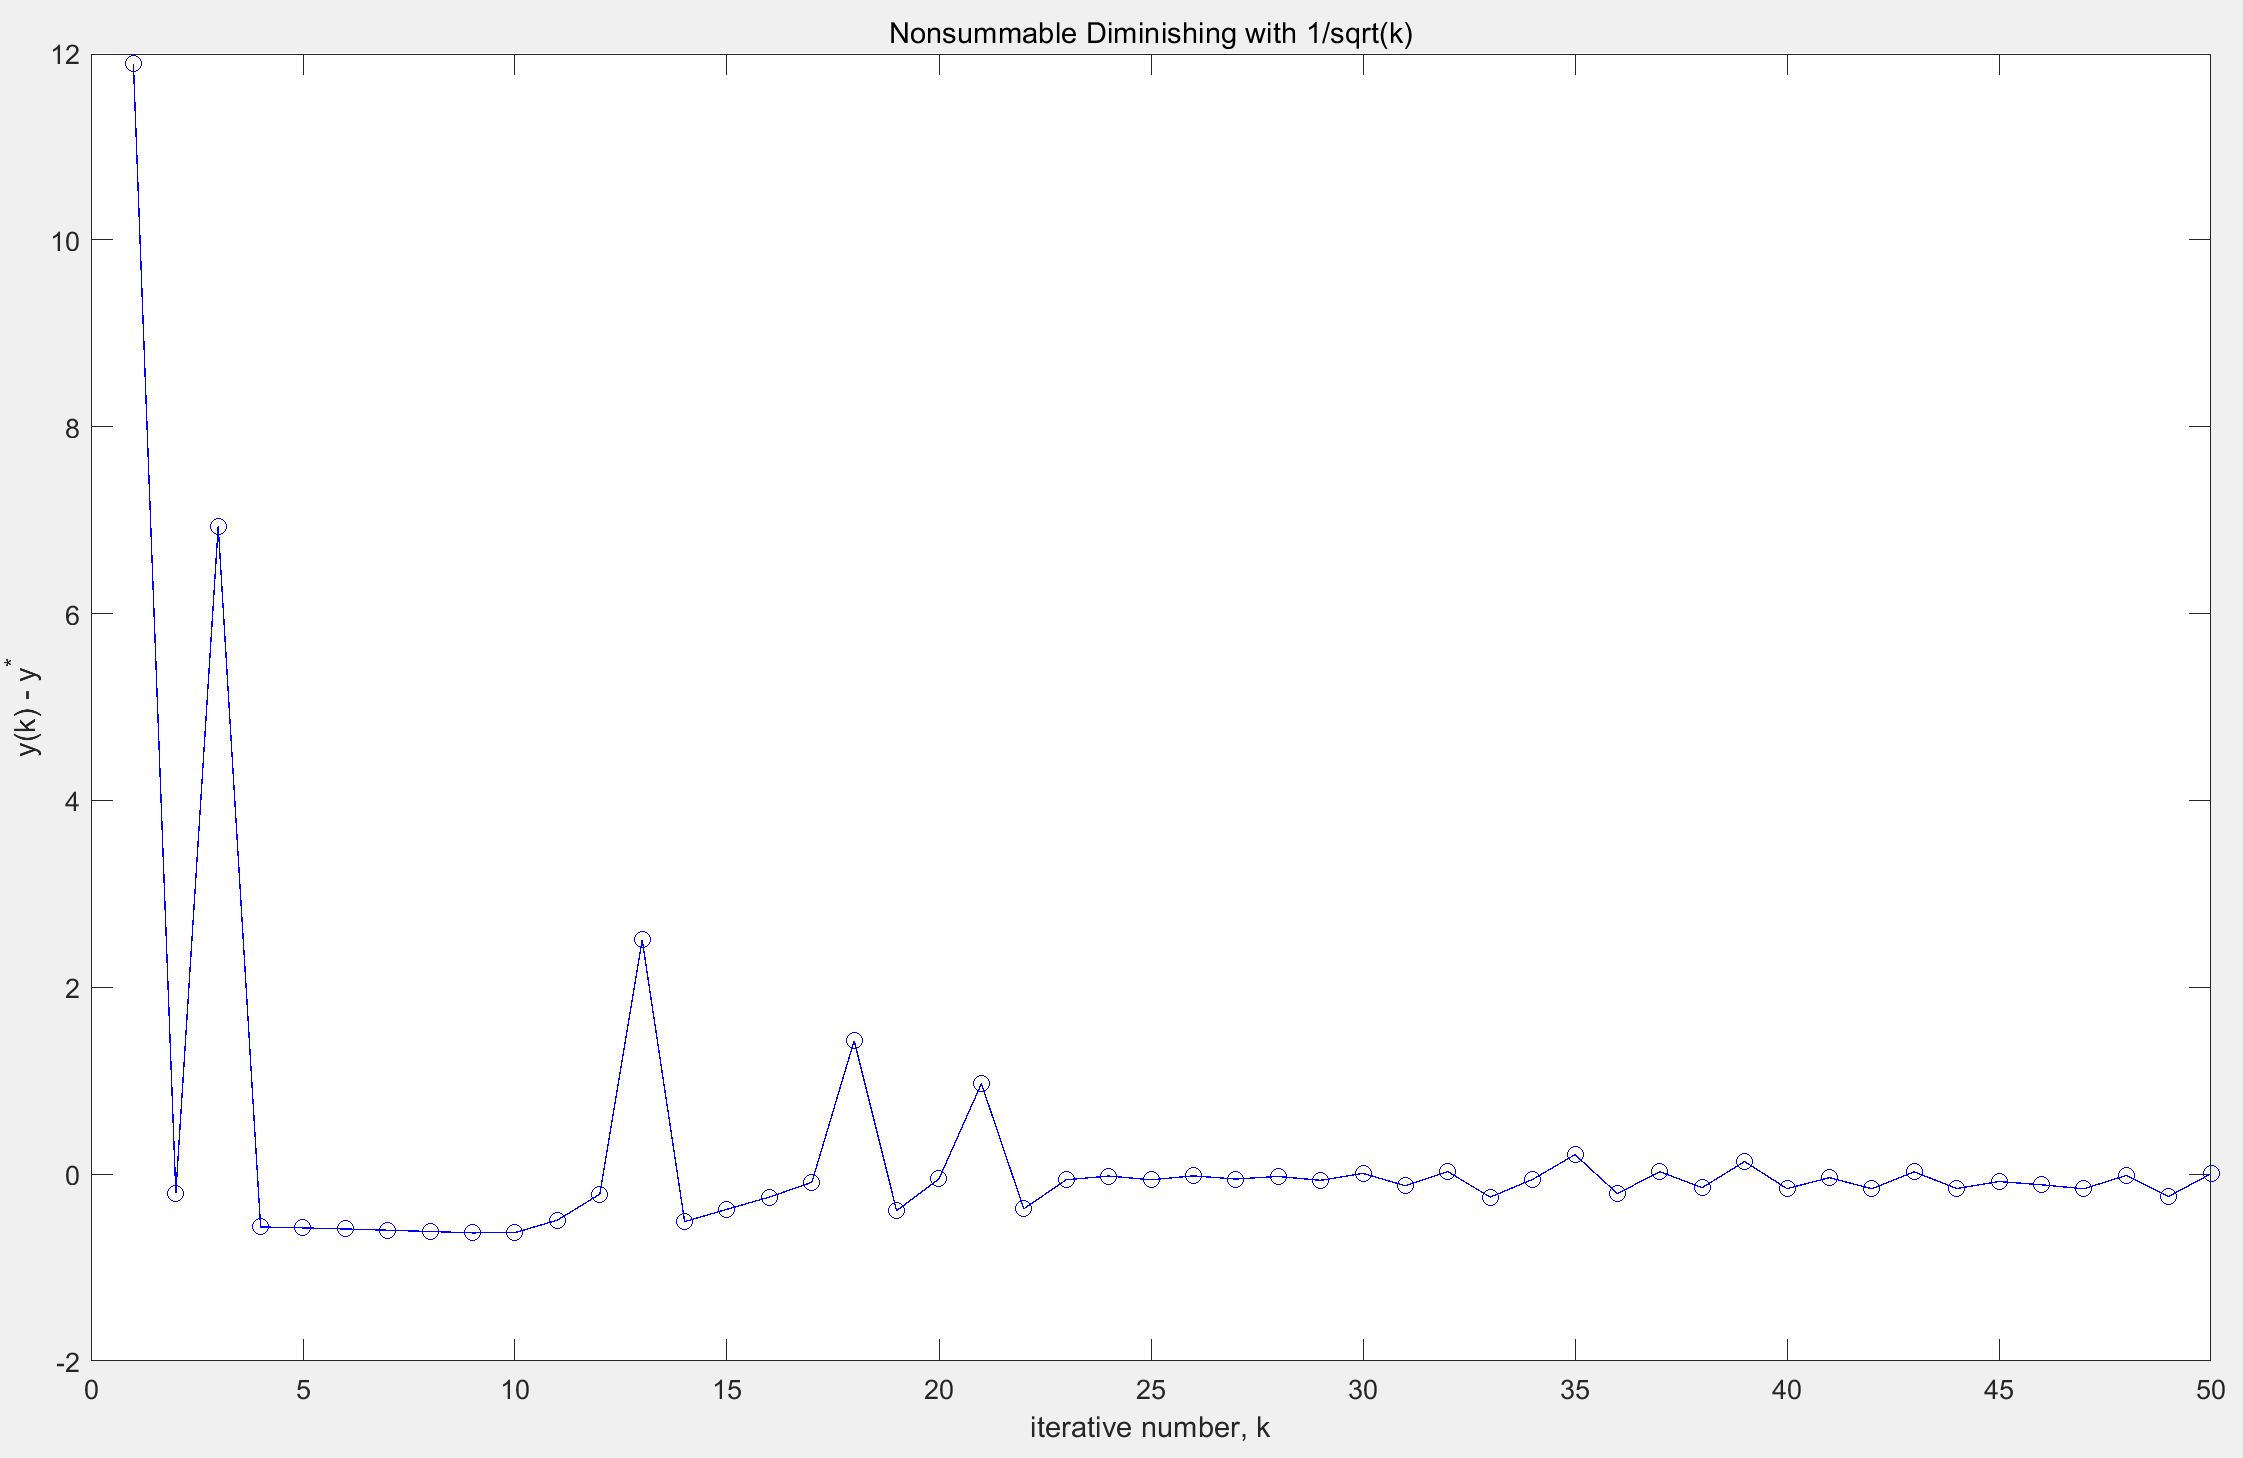
\includegraphics[width=1.0\textwidth]{img/a3+6(3).png}

    Polyak step: \\
    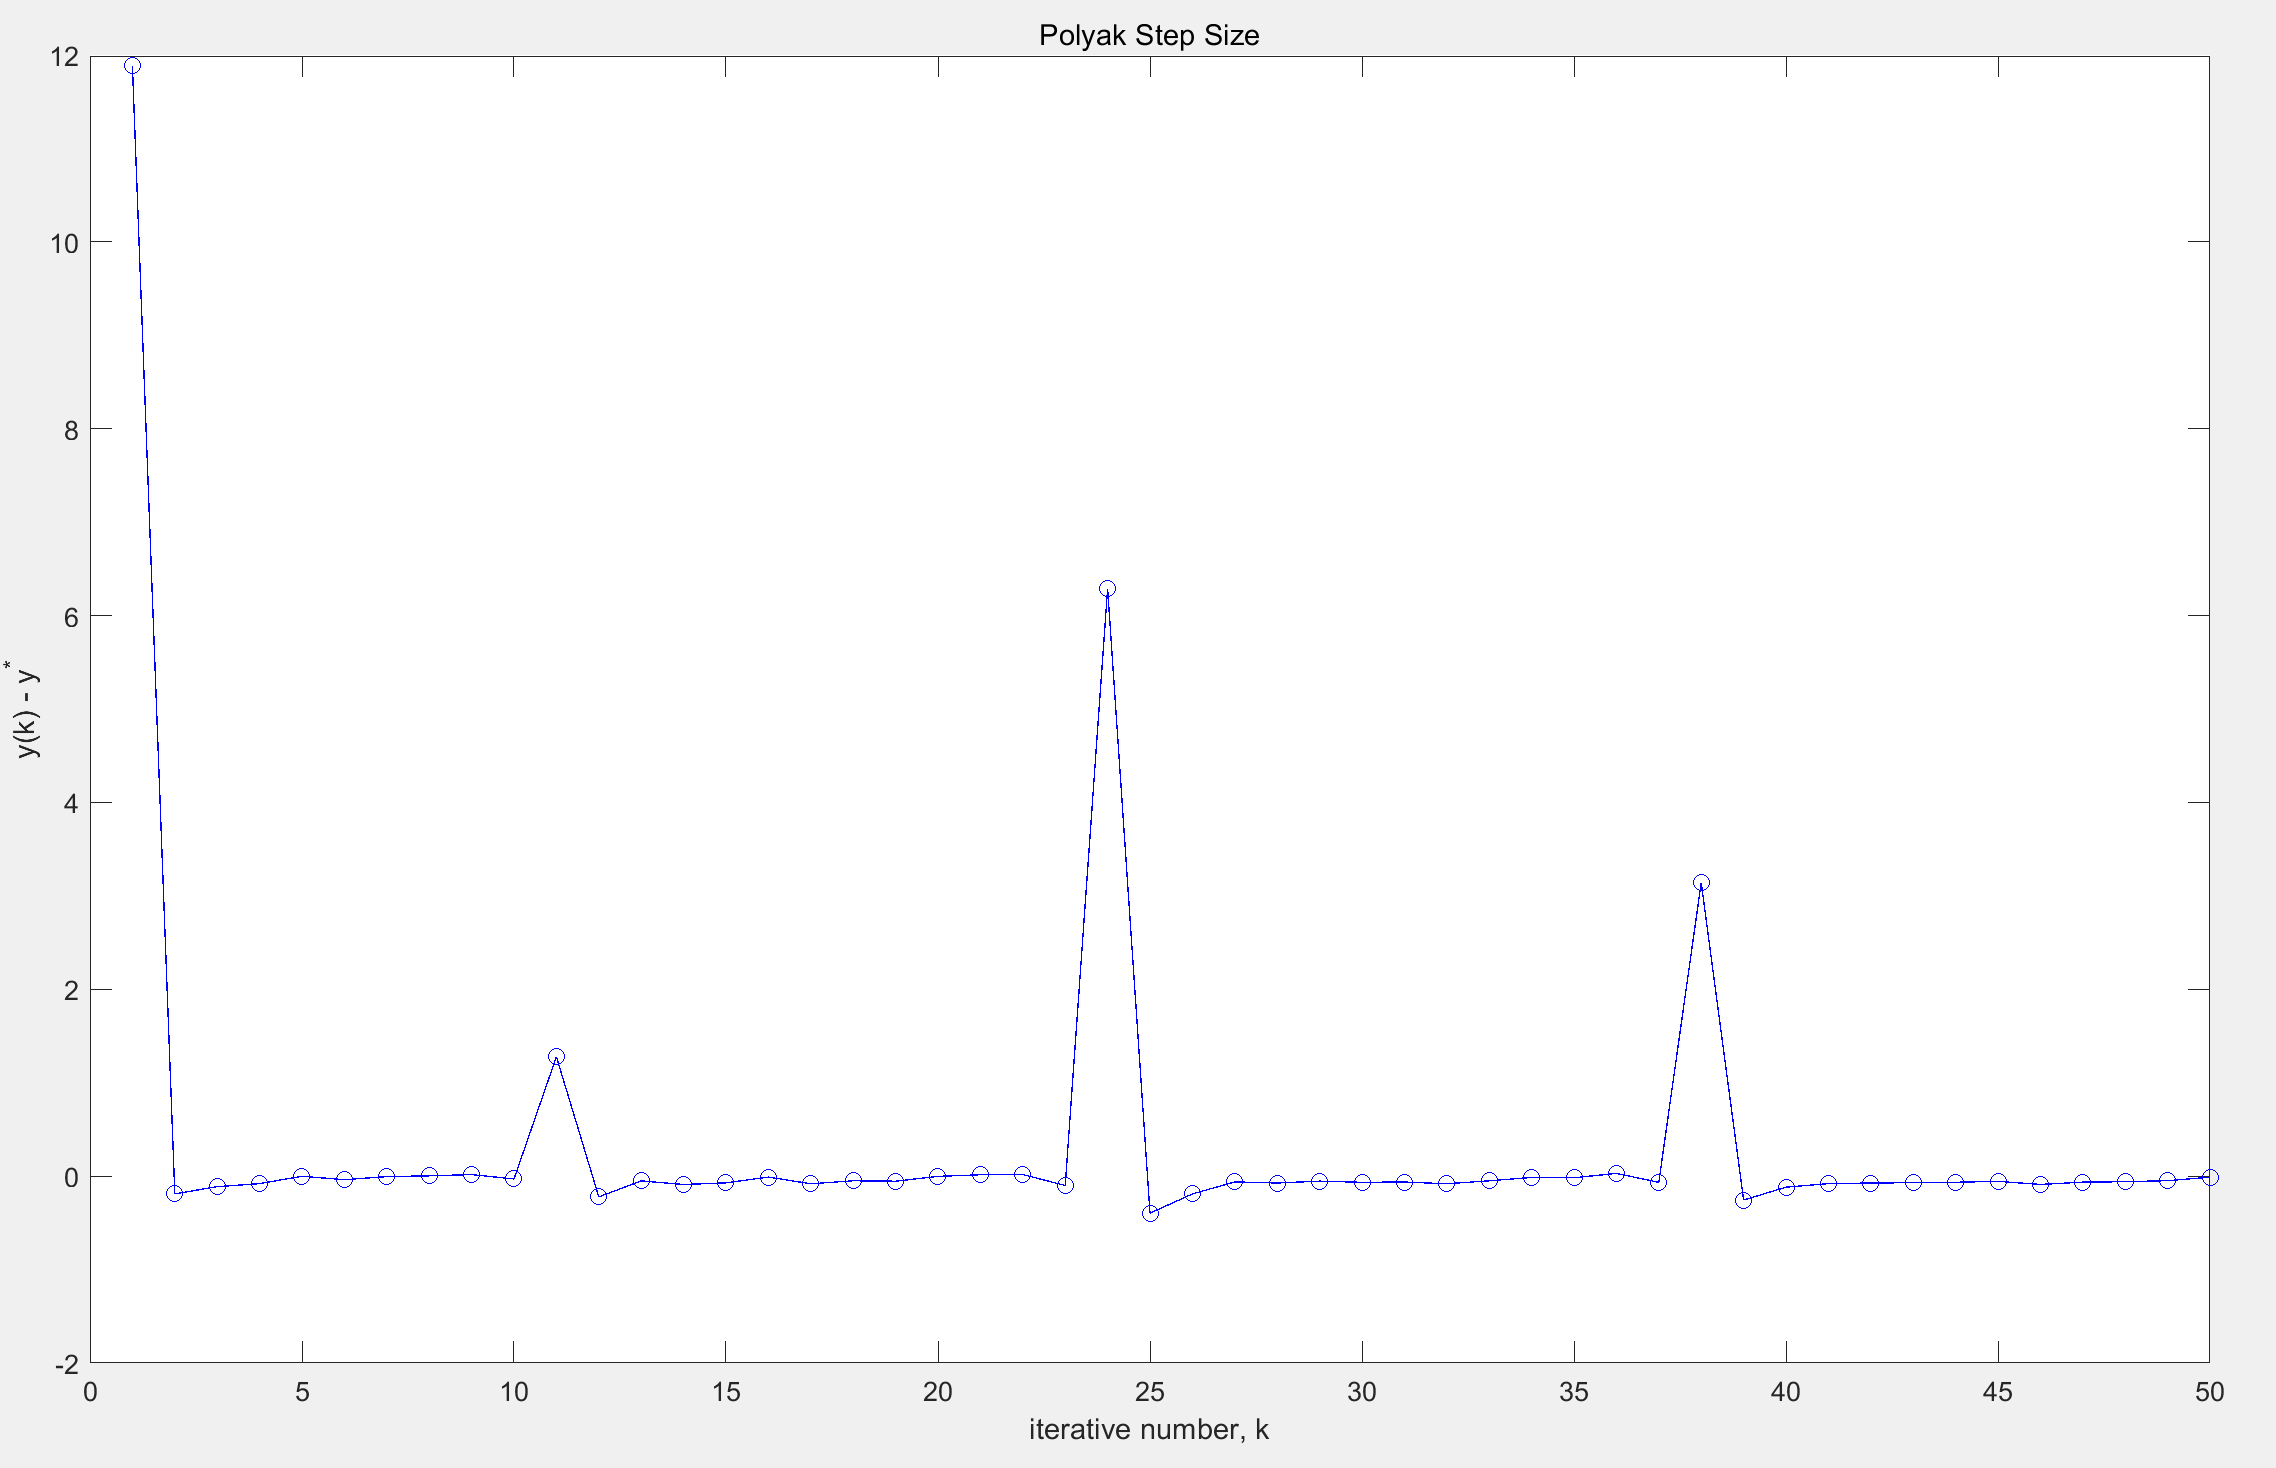
\includegraphics[width=1.0\textwidth]{img/a3+6(4).png}
\end{solution}

\end{document}